\documentclass{article}

\usepackage{tikz}
\usepackage{tkz-graph}
\usepackage{tkz-berge}

\begin{document}
\begin{center}
  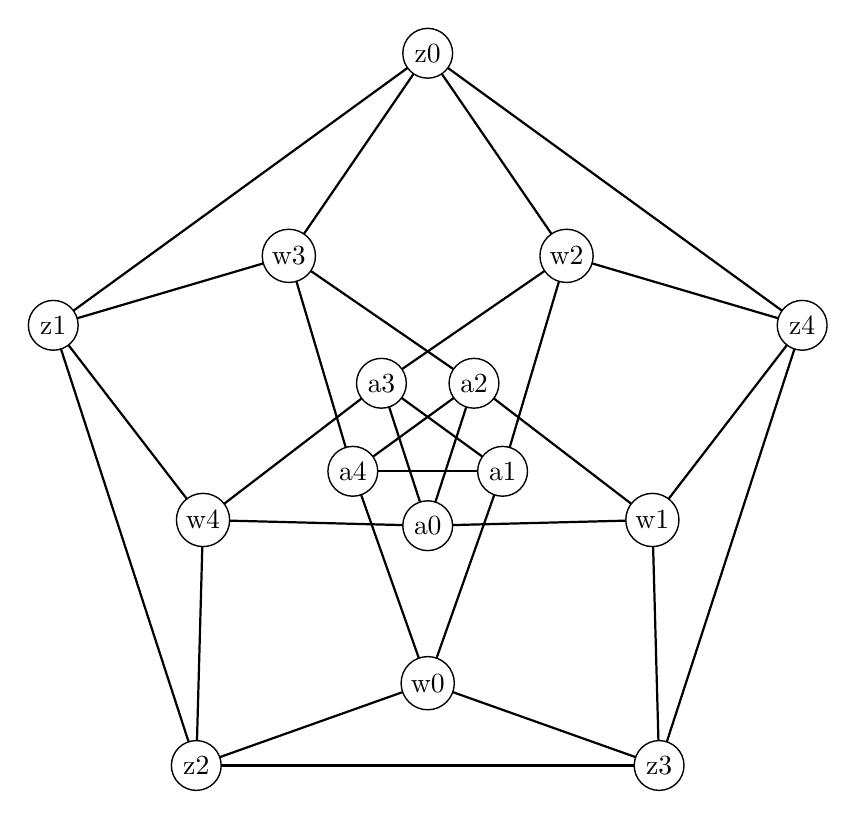
\begin{tikzpicture}
    \grEmptyCycle[RA=1,rotation=-90]{5}
    \grEmptyCycle[RA=3,prefix=w,rotation=-90]{5}
    \grCycle[RA=5,prefix=z,rotation=90]{5}
    \EdgeInGraphMod{a}{5}{2}
    \EdgeMod{a}{w}{5}{1}
    \EdgeMod{a}{w}{5}{-1}
    \EdgeMod{w}{z}{5}{2}
    \EdgeMod{w}{z}{5}{-2}    
  \end{tikzpicture}
\end{center}

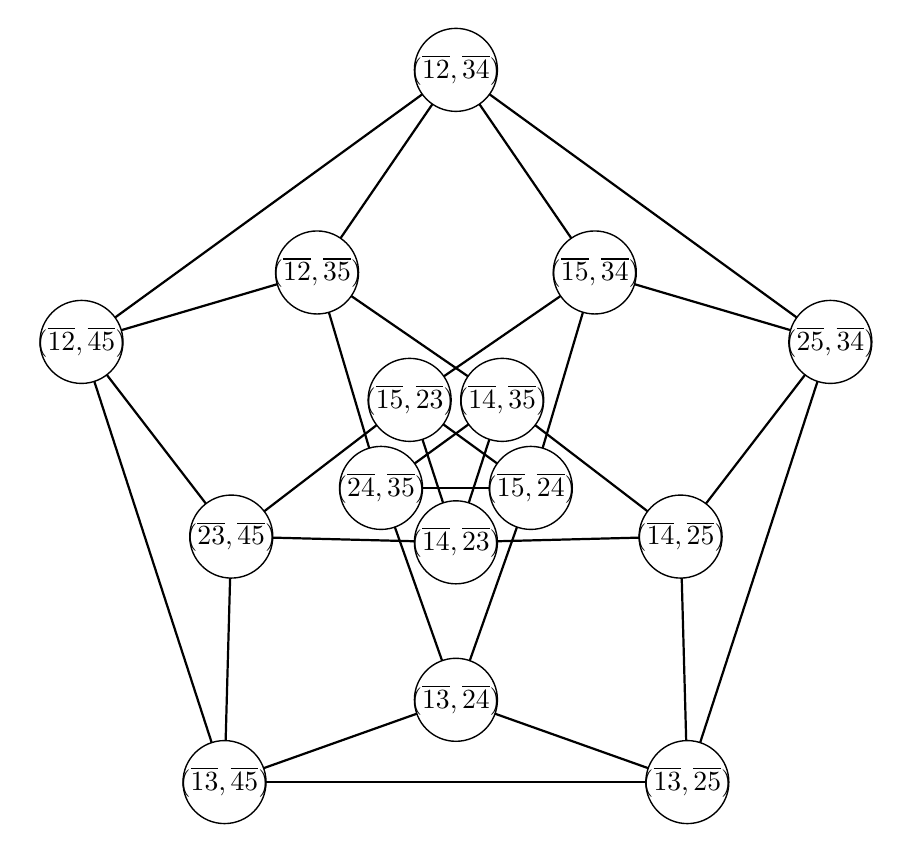
\begin{tikzpicture}%[rotate=90,scale=1]
  \newcommand{\aset}[2]{$\{#1,#2\}$}
  \GraphInit[vstyle=Classic]
  %\tikzset{VertexStyle/.style={draw,circle}}
  \SetVertexNoLabel
  \SetVertexMath
  \SetUpVertex[MinSize=30pt]
  \grEmptyCycle[RA=1,rotation=-90]{5}
  \grEmptyCycle[RA=3,prefix=w,rotation=-90]{5}
  \grCycle[RA=5,prefix=z,rotation=90]{5}
  \EdgeInGraphMod{a}{5}{2}
  \EdgeMod{a}{w}{5}{1}
  \EdgeMod{a}{w}{5}{-1}
  \EdgeMod{w}{z}{5}{2}
  \EdgeMod{w}{z}{5}{-2}   
  \AssignVertexLabel{z}{\textsl{$(\overline{12},\overline{34})$},\textsl{$(\overline{12},\overline{45})$},\textsl{$(\overline{13},\overline{45})$},\textsl{$(\overline{13},\overline{25})$},\textsl{$(\overline{25},\overline{34})$}}
  \AssignVertexLabel{w}{\textsl{$(\overline{13},\overline{24})$},\textsl{$(\overline{14},\overline{25})$},\textsl{$(\overline{15},\overline{34})$},\textsl{$(\overline{12},\overline{35})$},\textsl{$(\overline{23},\overline{45})$}}
  \AssignVertexLabel{a}{\textsl{$(\overline{14},\overline{23})$},\textsl{$(\overline{15},\overline{24})$},\textsl{$(\overline{14},\overline{35})$},\textsl{$(\overline{15},\overline{23})$},\textsl{$(\overline{24},\overline{35})$}}
\end{tikzpicture}
%\begin{center}
 % \begin{tikzpicture}
  %  \grEmptyCycle[RA=2,prefix=v,rotation=180,Math]{3} 
   %  \Edge[style={->}](v0)(v1)
    %\Edge(v1)(v2)
    %\Edge(a)(b)
  %\end{tikzpicture}
%\end{center}

\begin{center}
  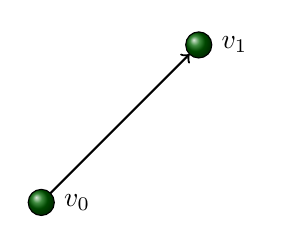
\begin{tikzpicture}
    \GraphInit[vstyle=Classic]
    \tikzset{VertexStyle/.style = {%
        shape= circle,
        shading= ball,
        ball color= green!40!black,%
        minimum size = 2pt,draw}}
    \Vertex[x=0,y=0,Math]{v_{0}}
    \Vertex[x=2,y=2,Math]{v_{1}}
    \Edge[style={->}](v_{0})(v_{1})
  \end{tikzpicture}
\end{center}

\begin{center}
  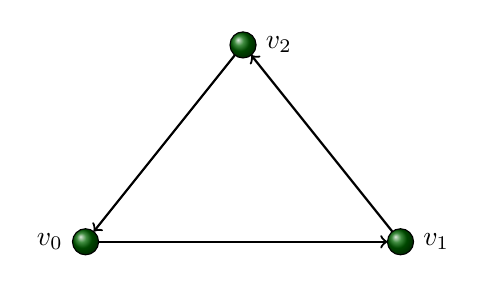
\begin{tikzpicture}
    \draw[help lines] (-2,0);% grid (2,3);
    %\SetGraphUnit{2}
    \GraphInit[vstyle=Classic]
    \tikzset{VertexStyle/.style = {%
        shape= circle,
        shading= ball,
        ball color= green!40!black,%
        minimum size = 2pt,draw}}
    \Vertex[x=-2,y=0,Math,LabelOut,Lpos=180,]{v_{0}}
    \Vertex[x=2,y=0,Math]{v_{1}}
    \Vertex[x=0,y=2.5,Math]{v_{2}}
    \Edge[style={->}](v_{0})(v_{1})
    \Edge[style={->}](v_{1})(v_{2})
    \Edge[style={->}](v_{2})(v_{0})
 \end{tikzpicture}
\end{center}

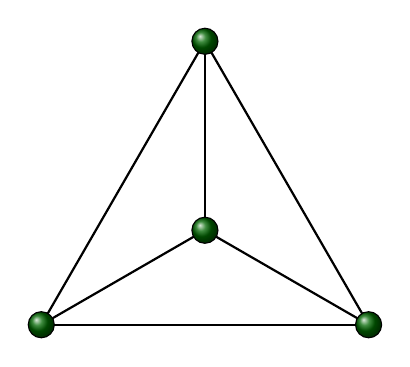
\begin{tikzpicture}[scale=.6]
  %\GraphInit[vstyle=Shade]
  %\renewcommand*{\VertexInnerSep}{4pt}
  \SetVertexNoLabel
  \GraphInit[vstyle=Classic]
    \tikzset{VertexStyle/.style = {%
        shape= circle,
        shading= ball,
        ball color= green!40!black,%
        minimum size = 2pt,draw}}
  %\SetGraphShadeColor{red!50}{black}{red}
  \grTetrahedral[RA=4]
\end{tikzpicture}

%\begin{center}
  %\begin{tikzpicture}
    %\grCycle[RA=3, style={thick,->}]
%    \Edge(a)(b)
 % \end{tikzpicture}
%\end{center}

\end{document}
